\tightsection{Motivation}

We first motivate the two key ideas of Dante:
(1) reducing streaming delay by replacing today's 
TCP-based streaming with retransmission-free FEC-based streaming, and 
(2) further improving quality using FOV-aware FEC coding.


\begin{figure}[t!]
	\centering
	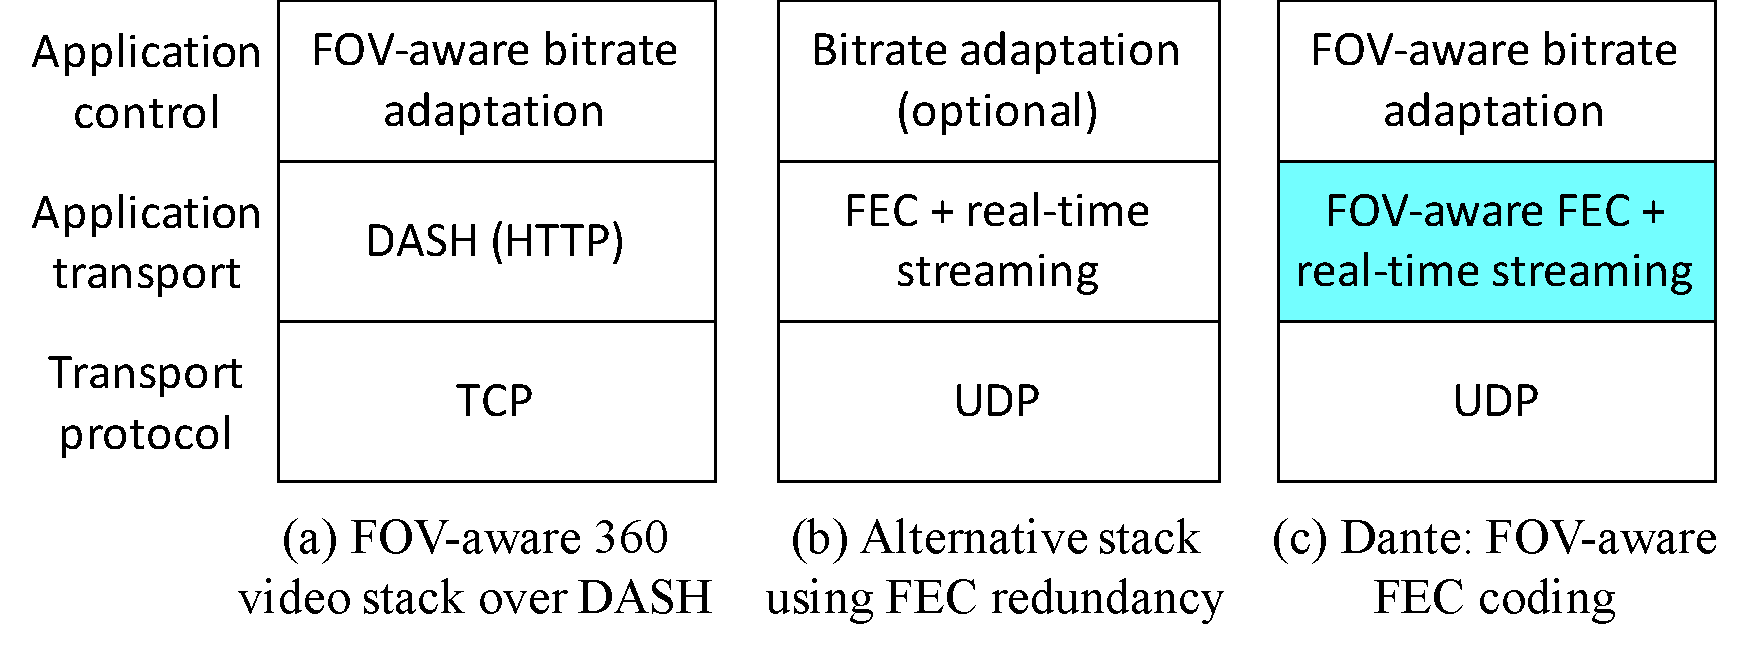
\includegraphics[width=0.5\textwidth]{paper_figs/dante-stack-comparison.pdf}
	\vspace{-0.5cm}
	\tightcaption{Contrasting Dante with previous solutions. 
	Dante proposes to replace the TCP-based streaming stack with 
	UDP-based FEC-enabled streaming stack to improve timeliness of 360-degree videos,
	and proposes to use FOV-aware FEC coding to further improve 
	delay-quality tradeoffs. 
	%\jc{This figure is still missing!!}
	}
	\label{fig:stack}
\end{figure}

We start with some background on 360-degree video streaming and 
the recent related work. In basic 360-degree video streaming, the 
server first encodes the video into 360-degree frames using standard 
video codecs (\eg HEVC~\cite{HEVC}) and streams them over TCP to the 
video player, which then plays the video in the region that the viewer
is currently watching, \ie FOV. Of course, this 
naive scheme works poorly in bandwidth-limited and error-prone 
wireless networks, because the available bandwidth can be less than 
what is needed for sending the 360-degree frames in their entirety. 


To address this issue, many recent work ~\cite{Viewport-adaptive,360ProbDASH,Adaptive_Streaming_Framework,Two-tier,Omnidirectional_Video_over_HTTP,Furion} propose 
to spatially partition each 360-degree frame to fine-grained 
``tiles'' (illustrated in Figure~\ref{fig:tile-based}), 
so that any FOV
of a viewer can be played by sending 
a small subset of tiles that cover the FOV, rather than the whole 
360-degree frame. This greatly saves bandwidth consumption. For 
instance, an FOV area typically spans 110 degrees horizontally and 
90 degrees vertically, so the fraction of video needed to cover FOV 
area is $\frac{{110^\circ }}{{360^\circ }} \times 
\frac{{90^\circ }}{{180^\circ }}{\rm{ = }}15{\rm{\% }}$ 
of the original 360-degree video. To leverage this observation, a 
common approach is to encode each tile in multiple bitrates, and in 
play time, the player predicts the FOV area and requests the tiles 
in different bitrate depending on how likely each tile falls in the 
FOV area. 

\begin{figure}[t]
		\centering
% 		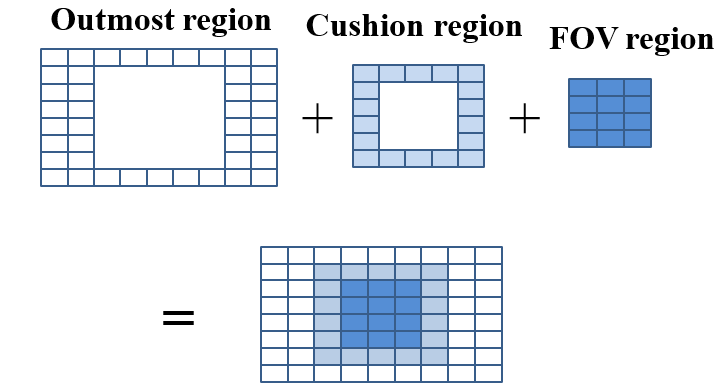
\includegraphics[scale=0.34]{paper_figs/tile_3_regions_0626.png}
        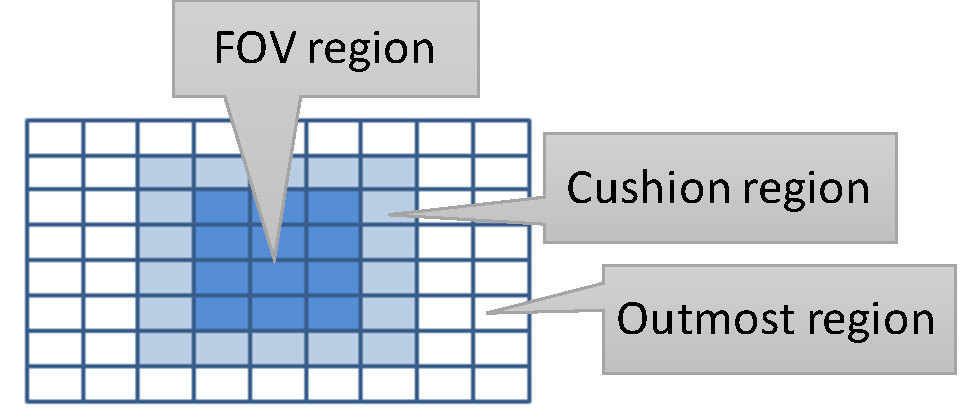
\includegraphics[scale=0.34]{paper_figs/dante-representation.pdf}
		\tightcaption{Tile-based representation of 360-degree video. Video 
		content in the FOV (field-of-view) region will be prioritized,
		\eg higher bitrate.}
%		\jc{please make it one line? don't call them "layers", call them "regions". }
		\label{fig:tile-based}
\end{figure}


\tightsubsection{Why FEC coding?}

Despite much bandwidth saving, these tile-based bitrate adaptive 
streaming techniques still use TCP (mostly via HTTP as an 
intermediate layer~\cite{MPEG-DASH}), and is ill-suited to streaming 
high-quality content while meeting constant and small streaming 
delay, because TCP is prone to be negatively affected by latency 
jitters and random packet losses, potentially causing interruptions
in video playbacks. Interruptions can cause viewers of 360-degree 
immersive videos to feeling dizzy~\cite{Simulator_Sickness}, 
so 360-degree videos are much more sensitive to 
playback interruptions than of traditional video content. The FOV-aware adaptive streaming schemes require system to prefeatch the video segment. However, it is difficult to accurately predict user's orientation
especially for long-term prediction (> 3s) \cite{360cellular}. Hence, the buffer length should be not greater than 3s so as to guarantee the quality of the video fraction users are actually watching.


%\jc{add some concrete numbers on how much short the latency needs to be and provide citations/references. }

Instead of using retransmission to provide reliability, we consider
an alternative approach that uses FEC 
code to deliberately introduce a controlled amount of redundancy, so 
that a small number of packet losses can be recovered without 
retransmission. FEC-enabled protocols (\eg RTP~\cite{rfc5109}) are often 
used to support delay-sensitive video streaming over UDP
(\eg video conference). 

The basic idea behind using FEC in video streaming is as follows. 
If a video segment includes $K$ uniform-sized data packets, the FEC 
encoder then takes these packets as input and adds $A$ ``repair 
packets'' to create a coded block of size ${{B = K + A}}$. And we assume the packet size is equal to Maximum Transmission Unit (MTU). These redundant repair packets allow the receiver to recover the origin $K$ packets, as long as at least {\em any} $K$ of the ${K + A}$ 
packets are received.\footnote{It is worth noting that the FEC in 
this paper operates at the level of data packets, rather than bits.
That is, we do not add redundancy to each individual packet (as in 
some link-level protocols); instead, we apply FEC coding to 
generate redundant packets of a given group of packets to tolerate
any packet-level losses.} The redundancy of FEC is defined by 
${A/K}$. Obviously, one can tolerate more packet losses by using a 
higher FEC redundancy. 
%\jc{make sure the math notions, B, K, A are not used in other sections, or are used with the same physical meaning}
	
A critical question is whether the benefit of FEC coding (\ie less
latency) outweighs its cost (\ie increased data sizes).
Figure~\ref{fig:goodput_redundancy} shows the impact of the FEC redundancy on the video
streaming goodput---the amount of video data (after FEC decoding) 
received within a fixed delay (1s) after it is sent out. The network parameter set is seen in section 4.
%\jc{what's the set up here? you can add a forward pointer to eval if it's the same set up you will explain there. what data was used to generate the graph? what's the delay constraint? how was the network condition (pkt loss rate, delay)?}
As FEC redundancy increases, at first the goodput 
does increase, since a bit redundancy improves robustness against 
packet losses. The goodput peaks at FEC redundancy of 3\%,  and then begins to
drop with higher FEC redundancy, 
as too much redundancy starts to cause self-inflicted congestion.
The important takeaway here is that setting a suitable value of FEC 
does improve video streaming quality by striking the balance between
robustness against packet losses and throughput. 

\begin{figure}[t]
	\centering
	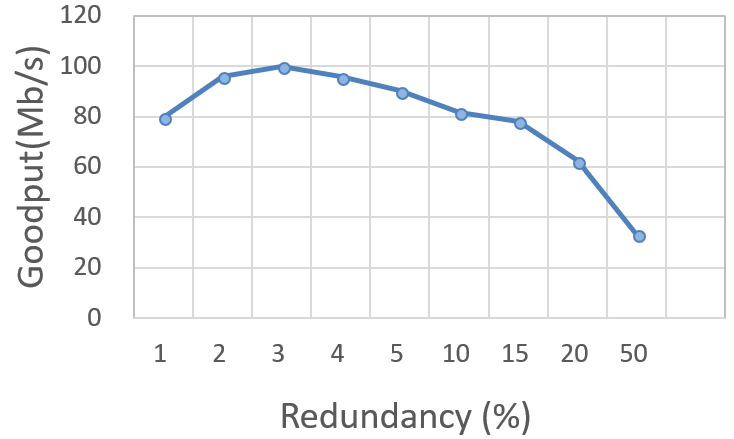
\includegraphics[scale=0.32]{paper_figs/goodput_With_redundany_big_font.png}
	\tightcaption{The impact of various FEC redundancy on video streaming goodput.}
	\label{fig:goodput_redundancy}
\end{figure}


\tightsubsection{Why FOV-aware FEC?}
By replacing the TCP-based streaming protocol in 360-degree videos 
with UDP-based and FEC-enabled protocols, we not only reduce 
streaming delay, but 
introduce a new opportunity as well---one can further improve 
FEC-enabled streaming protocol by taking advantage of the 
fact that the viewer's attention is not uniformly spread, 
but focuses on FOVs.

Figure~\ref{fig:example} 
shows an example of this opportunity in action. We
consider two spatial regions in the same 360-degree video segment, 
one in the FOV region, and the other in the non-FOV region, and we use 
two strategies to set FEC redundancy, one unaware of FOV (giving 
equal FEC redundancy to both regions) and the other aware of FOV (\ie 
giving a better FEC redundancy to the FOV region than the non-FOV 
region). In this example, we set packet loss rate to be 1\%,
network capacity 40Mb/s, video segment length 0.5 second, the delay constraint is 500ms, i.e., the video segment should be encoded by FEC encoder of the server side, then sent, received and finally decoded by FEC decoder of the client side within 500ms, the size of FOV region
4Mb, and the size of non-FOV region 2Mb (\eg application assigns 
a lower bitrate to the non-FOV region, but this doesn't affect our 
observation). We use PSNR ~\cite{Viewport-adaptive} to measure the video quality by calculating the effect the noise caused by information loss has on video fidelity. The higher is video's PSNR, the better is it's quality. 
%\jc{how exactly this is done?}
Now, compared to applying FEC redundancy of 3\% to both regions, 
if one apply 5\% to the FOV region and 2\% to the non-FOV region, 
the resulting video quality in the non-FOV region will be almost the 
same (with a marginal 5.7\% drop), but the video quality in the
FOV region is significantly improved by 23\%. 
Note that 23\% is a significant improvement,
given PSNR is in log scale. 
%\jc{say something like: 23\% is significant because psnr is in log scale, etc}
%\jc{what does 23\% higher PSNR mean physically? can you find some quote? 我查了相关的文献,暂时没有找到具体的解释}

% We find that, instead of different regions encoded with the same 
% FEC redundancy, it can lead to the better video quality that 
% different regions are encoded with different FEC redundancy 
% before the transmission.

\begin{figure}[t!]
	\centering
	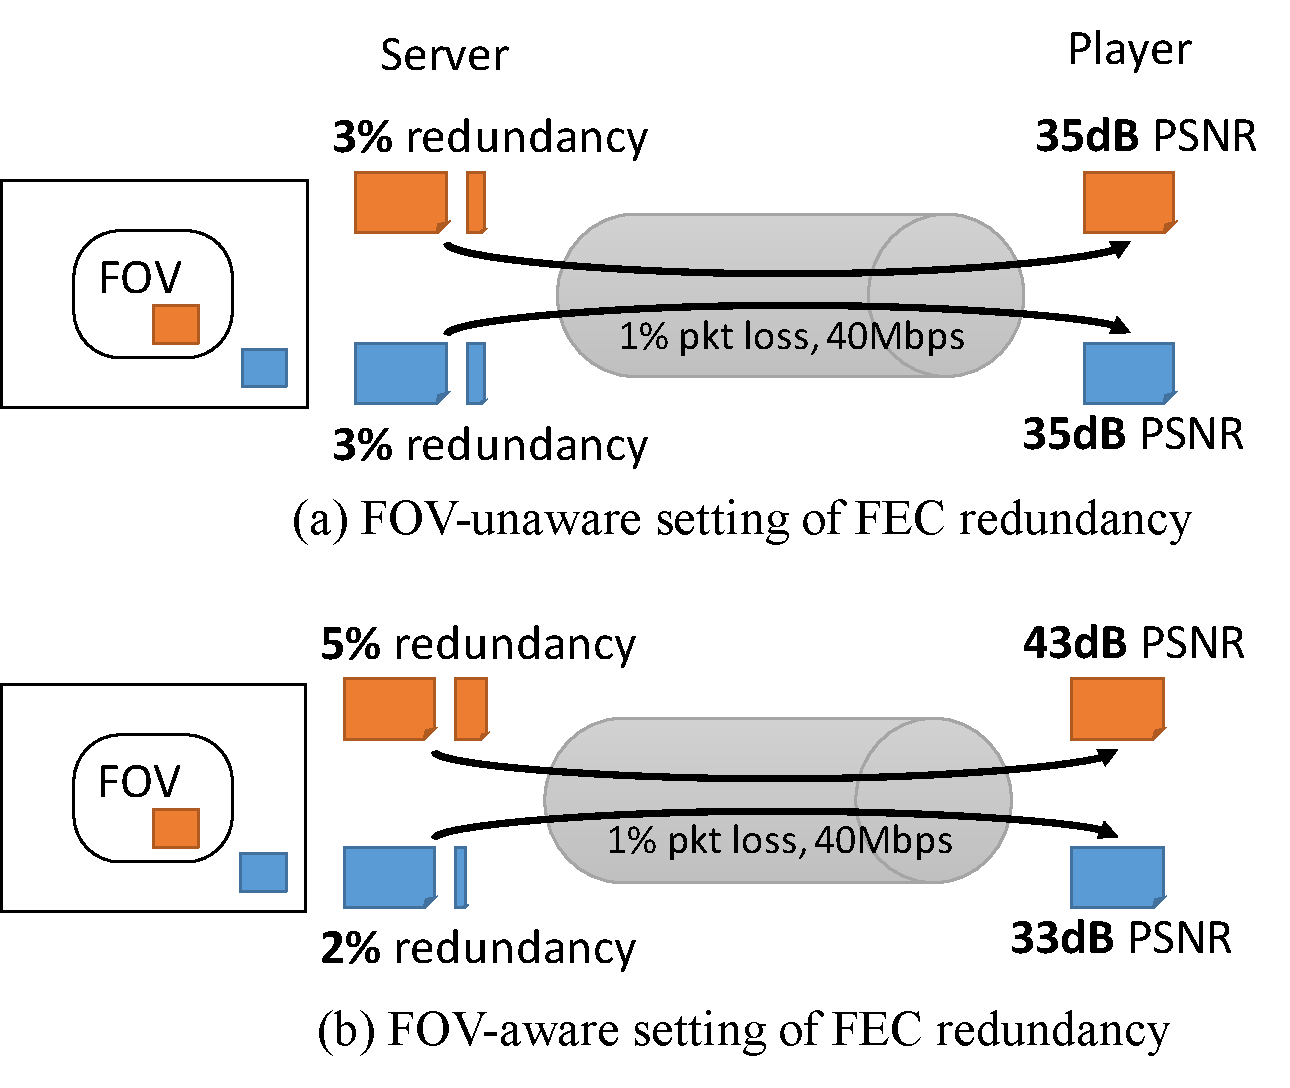
\includegraphics[width=0.36\textwidth]{paper_figs/dante-fec-example.pdf}
	\tightcaption{An illustrative example that setting FEC redundancy based on FOV can significantly 
	improve video quality in the FOV regions.}
	\label{fig:example}
\end{figure}
	
% 	\begin{table}
% 		\centering 
% 		\scriptsize
% 		\begin{tabular}{p{2.0cm}p{2.0cm}p{1.6cm}p{1.6cm}}
% 			\rowcolor[gray]{0.9} 
% 			\hline
% %			 The length of segment &The size of QER region(Mb) & The size of non-QER region(Mb) &
% 			The FOV redundancy(\%) &The non-FOV redundancy(\%) & Expected PSNR of FOV(dB) & Expected PSNR of non-FOV(dB)\\
% 			\hline
% 			3  &  3  &  35  &  35\\    
% 			\hline
% 			2  &  5  &  43  &  33\\ 
% 			\hline
			
% 		\end{tabular}
% 		\caption{The Video Quality of different FEC redundancy combinations}
% 		\label{}
% 	\end{table}

% Finally, note that our approach is complementary to the 
% application-layer tile-based bitrate adaptation: given any 
% selection of tile and bitrate, we apply FEC coding to improve
% timeliness of streamed content by avoiding resending data 
% packet as in TCP.